There are many ways to open the \textbf{Create Projection} tool.  This section assumes that you have loaded multiple layers and wish to batch project them; therefore, we will use this as the starting point to creating a projection.

\begin{enumerate}
	\item Open the \textbf{Batch Project} tool from the Arc Toolbox.  \textbf{Arc Toolbox} $\rightarrow$ \textbf{Data Management Tools} $\rightarrow$ \textbf{Projections and Transformations} $\rightarrow$ \textbf{Feature} $\rightarrow$ \textbf{Batch Project}
	\item Add all the layers as input
	\item Choose an \emph{Output Workspace} (preferably a new directory with the projection in its name)
	\item The \emph{Output Coordinate System} input will open the window shown in figure \ref{create_proj_1}, choose New $\rightarrow$ Projected \\
	At this point you should be at the window shown in figure \ref{create_proj_2}
	\item Choose the values shown in figure \ref{create_proj_2}, \ie \begin{itemize}
		\item False Easting: \textbf{0.0}
		\item False Northing: \textbf{0.0}
		\item Central Meridian: \textbf{-97.0}
		\item Standard\_Parallel\_1: \textbf{33.0}
		\item Standard\_Parallel\_2: \textbf{45.0}
		\item Latitude\_Of\_Origin: \textbf{40.0}
		\item Linear Unit: \textbf{Kilometre}
		\item Geographic Coordinate System: \textbf{GCS\_North\_American\_1983} \\
		\item[Note:]  WGS84 is effectively identical to NAD83 for the purposes of this tutorial, but if WGS84 is chosen you will then be required to enter a transformation (NAD83\_to\_WGS\_1984\_1) when projecting.  This is also uncertain, as other people have suggested that \acs{cmaq} uses a sphere projection\footnote{\url{https://dawes.sph.unc.edu/groups/project\_users/revisions/d7557/4/}}.
	\end{itemize}
	\item Press \textbf{Save as\ldots} to save the projection
\end{enumerate}

\begin{figure}
	\centering
	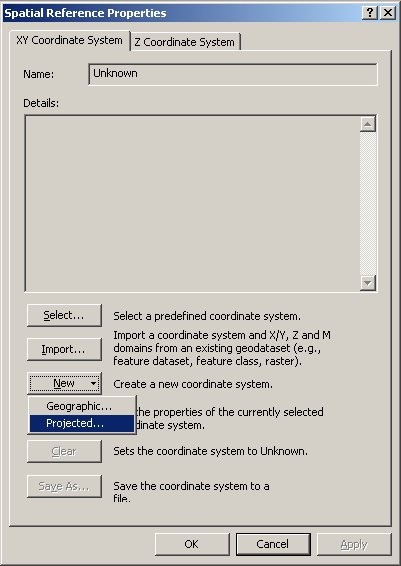
\includegraphics[width=0.50\textwidth]{create_projection_1.jpg}
	\caption{Select Projection Dialog}
	\label{create_proj_1}
\end{figure}

\begin{figure}
	\centering
	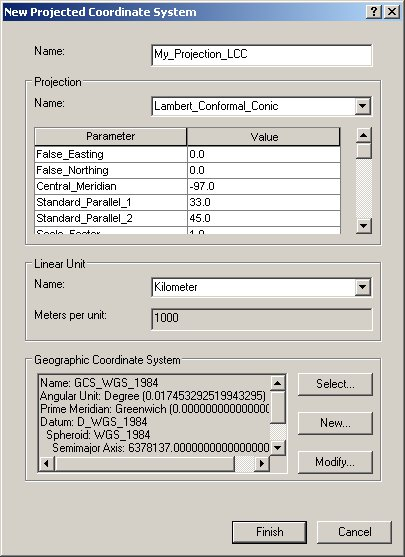
\includegraphics[width=0.50\textwidth]{create_projection_2.jpg}
	\caption{Create Projection Dialog}
	\label{create_proj_2}
\end{figure}

Project the data, then load all the data into a new data frame.


